\documentclass[border=5mm]{standalone}

\usepackage{pgfplots}
\usepgfplotslibrary{polar}
\begin{document}

 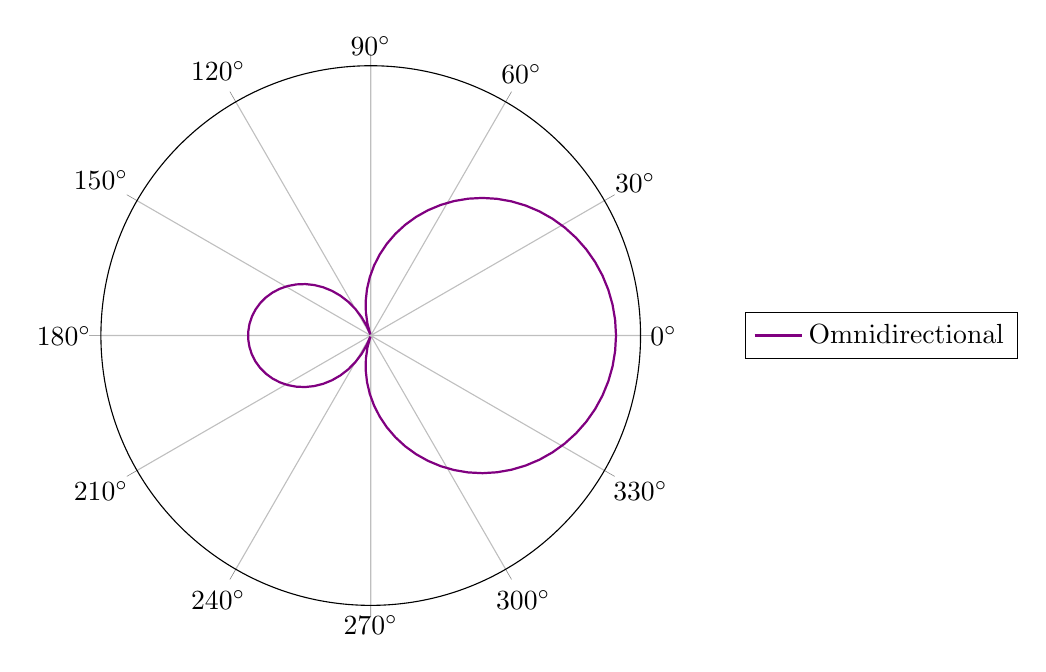
\begin{tikzpicture} % p56
    \begin{polaraxis} [
            ytick=\empty,
            hide y axis,
            xticklabel=$\pgfmathprintnumber{\tick}^\circ$,
            legend entries={
                Omnidirectional,
                Figure-8,
                Subcardioid,
                Cardioid,
                Supercardioid,
                Hypercardioid
            },
            legend cell align=left,
            legend style={
                at={(1.7,0.5)},
                anchor=east
            },
            every axis plot/.style={
                thick,
                samples=100,
                domain=0:360
            }
        ]
        %Ominidirectional
%    \addplot[black]{1};
%        %Figure 8 (Bidirectional)
%    \addplot[blue]{abs(cos(x))};
%        %subcardiod
%    \addplot[green]{0.7 + 0.3*cos(x)};
%        %cardiod
%    \addplot[brown]{0.5 + 0.5*cos(x)};
%        %Supercardioid
%    \addplot[red]{abs(0.37 + 0.63*cos(x))};
        %Hypercardioid
    \addplot[violet]{abs(0.25 + 0.75*cos(x))};
    \end{polaraxis}
\end{tikzpicture}
\end{document}